\chapter{Baseband Filter}%
\section{Filter Specifications}%
Baseband filter is the first block after the mixer and it's 
main poprpuse is to reject the in-band blocker at 300MHz, a 
second mode should be added to the filter in-order to work 
for DPD (600MHz),
Here are the specifications shown in 
Table~\ref{tab:filter_specs} 
\begin{table}[htpb]
    \centering
    \caption{Baseband filter specifications}
    \label{tab:filter_specs}
    \begin{tabular}{|c|c|}
        \hline
        Paramter& Value  \\ \hline
        Bandwidth (0.5dB) & 250MHz \\ \hline
        Rejection at (300MHz) & 30dB \\ \hline
        Gain & 0dB \\ \hline
        NF  & 12 dB \\ \hline
        OIP3 & 16dBm \\ \hline
        OIP2 & 55dm \\ \hline
        3dB-Bandwidth (Mode 2) & 600MHz \\ \hline
    \end{tabular}
\end{table}


\section{Literature Review}%

\subsection{Performance Metrics for baseband filters}%
\subsubsection{Rejection}%
It's clear that the most imporntant metric of a filter is 
how much rejection it provide to the unwanted signal.
\subsubsection{Pass-band Bandwidth}%
Bandwidth of the filter is also very important metric, it should 
be greater than or equal to the channel BW but not very high to
reduce noise and power.
\subsubsection{Group delay of the filter}%
Group delay (eq~\ref{eq:group_delay})  is the measure of linearity
of the phase response , a constant group delay indicates a linear
phase response , meaning oall the signal components has the 
same delay \cite{Saari2012} ,in our case it's not very critical since group delay variation can be compensated in digital domain.
\begin{equation}
    GD = \frac{d\phi}{dt}
    \label{eq:group_delay}
\end{equation}

\subsubsection{Input referred Noise}%
Input referred noise shouldn't be very high in order to maintain
good SNR , The degradation of Receiver noise figure due to
baseband noise is given by eq~\ref{eq:noise_RX_baseband} \cite{Saari2012}
\begin{equation}
    NF_{RX} = 10 \log(10^{NF_{RF}/10} + 
    \frac{v_{n\,in\,BB}^2}{k T B_{RF}\ RS\ (AV_{RF})^2})
    \label{eq:noise_RX_baseband}
\end{equation}
Noise figure of the filter itself is given in Table~\ref{tab:filter_specs} NF = 12dB, relation between Noise figure and input 
referred noise is given by eq~\ref{eq:noise_figure_input_noise}
\begin{equation}
    NF = 10\log(1+ \frac{V_{n\, in}^2}{4KT\ R_S \ BW})
    \label{eq:noise_figure_input_noise}
\end{equation}

\subsubsection{Linearity}%
Non-linear distortion caused by inter-modulation products and 
compression is very critical in our system specailly for this 
filter since this is where the blocker should be filtered, 
for our system required OIP3 = 16dBm.

\subsection{Types of Filters}%
\subsubsection{Passive and Active filters}%
Filters can be catogrized into two main catagories: Passive filters
and Active filters.

Passive filters are very linear (since it's passive) and
consumes no power but offers 
no gain and very large at low frequencies.\\
On the other hand, active filters are more suitable for 
low frequencies , but  have power consumption, the impelemented 
filter in this system is an active filter

\subsubsection{Filter Approximations}%
An Ideal filter is like Break-wall , passes all frequencies in 
the Pass-band and reject frequencies in stop bands completely,
there are several filter types that approximates this behavior.
\subsubsection{Butterworth filter}%
Butterworth or maximally flat response is an approximation that 
achieve maximum pass-band flatness , has no pass-band ripples but
has poor rejection for a given order, filter Transfer function is 
given eq~\ref{eq:butterworth_TF} , where n is the order , 
$\omega_c$ is the cutoff frequency and $\omega$ is the frequency
in rad/s.
\begin{equation}
    |H(j\omega)|^2 = \frac{1}{1+(\frac{\omega}{\omega_c})^{2n}}
    \label{eq:butterworth_TF}
\end{equation}
\subsubsection{Cheybeshave filter}%
Chebyshev filters gives a better roll off in the cost of pass-band
ripples and Group delay variation.
\subsubsection{Bessel filter}%
Bessel filter has the worst roll-off (rejection) of all filter 
types , but offers very linear phase variation (constant group 
delay)
\subsubsection{Elliptic filter}%
Elliptic filter gives the steepest roll-off (stop-band rejection)
but offers a very bad group delay variations, also Elliptic
approximation has transmission zeros in its transfer function.

\subsubsection{Active filters Impelementations}%
There are mainly to approaches for impelementing active filters:
using Bi-quad sections or LC-ladder simulation.\\
For the Bi-quad sections impelementations are sallen-key ,
Multiple-feedback , etc. these sections are suitable for low 
quality poles and low order filters because it has high components
sensitivity. \\
On the other hand LC-ladder simulation offers low components 
sensitivity, there are two types of LC-ladder simulation one
is called leap-frog which is based on integrators and the other
is based on gyrators that simulate that transfer charactristics of
inductors.

\subsubsection{OPamp-RC Vs GM-C filters}%
OPamp-RC technique is based on OPamps with RC feedback , this 
technique is usaully linear (because of feedback) and its noise
performance determined by the resistance , but since it depends
on feedback it's not very good at high frequencies because of 
stability.

GM-C technique is based on OTA rather than full OPamp also it's 
an open-loop technique this means it can work for higher frequency
(no stability consedrations) , but it has a poor linearity.
\cite{Saari2012_ch3}

\section{Design Methodology}%
\subsection{Filter Approximation}%
Given Rejection and Bandwidth in Table~\ref{tab:filter_specs},
we can choose filter approximation based on filter order that
achieves the specifications, 
From results shown in Table~\ref{tab:filter_approx_tabel}, elliptic
filter approximation is chosen, Magnitude response of this 
filter is shown at Figure~\ref{fig:Filter_Response_first} , this
is the original elliptic filter response  , the highest quality
factor of the poles is 8.9 , this is important since we will need
in filter impelementation.
\begin{table}[htpb]
    \centering
    \caption{Filter Approximations order}
    \label{tab:filter_approx_tabel}

    \begin{tabular}{|c|c|}
        \hline
        Approximation Type & order  \\ \hline
        Butterworth & 25 \\ \hline
        Chebyshev 1 & 9 \\ \hline
        Elliptic & 5 \\ \hline
    \end{tabular}
\end{table}

\begin{figure}[htbp]
  \centering
  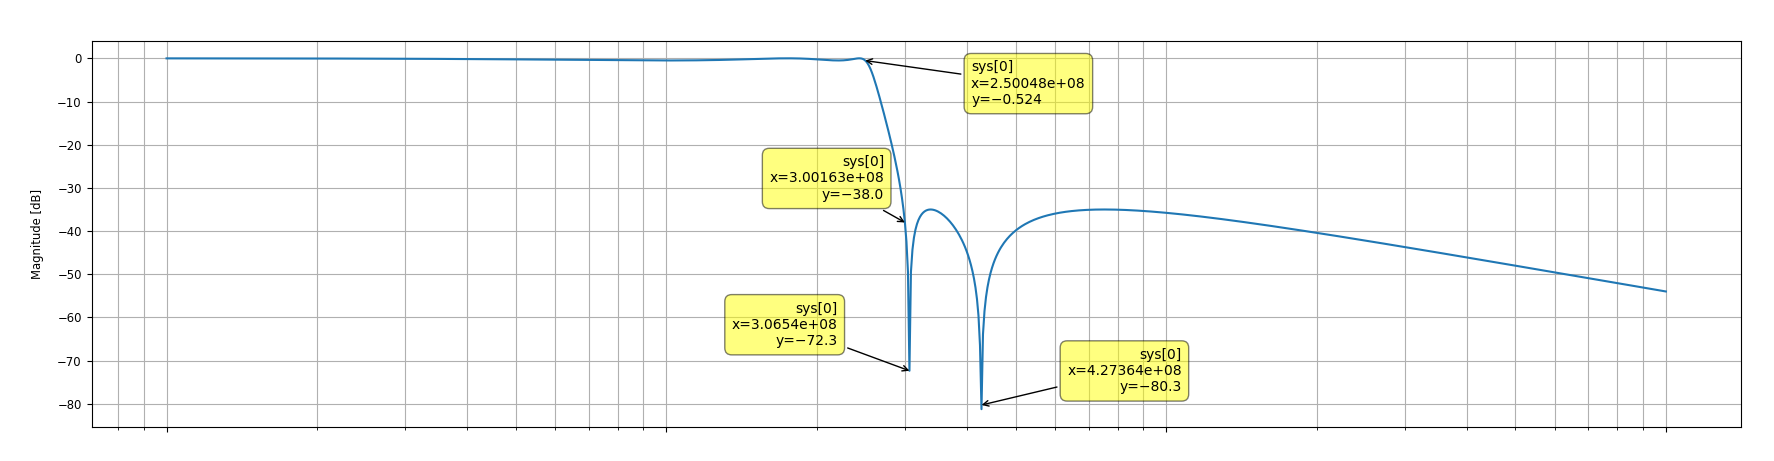
\includegraphics[width=1\textwidth]{images/Filter_Response_first.png}
  \caption{Elliptic Filter Magnitude Response}
  \label{fig:Filter_Response_first}
\end{figure}

This filter approximation is changed later  to compensate losses
and non-idealities of the actual impelementation , the final 
filter approximation compared with original one in pole-zero map
is shown in Figure~\ref{fig:final_approx_Vs_orignal}, note that
maximum pole quality factor is 6.2

\begin{figure}[htbp]
  \centering
  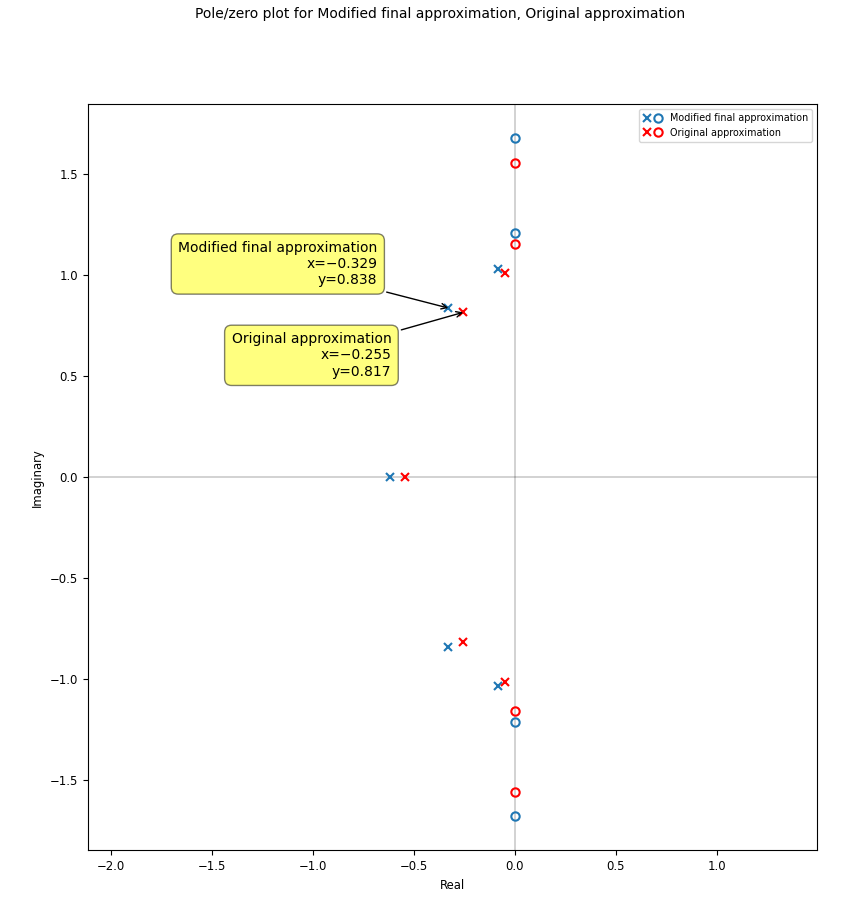
\includegraphics[width=0.8\linewidth]{images/final_filter_approx_Vs_orignal_pzmap.png}
  \caption{Modified filter approximation Vs original pole-zero map
  }
  \label{fig:final_approx_Vs_orignal}
\end{figure}
\clearpage

\subsection{Impelementation technique}%
\label{sub:Impelementation technique}
After we chose filter approximation , a suitable impelementation
technique is required ,as discussed in Literature since we are 
at baseband passive LC-ladder impelementation  is not possible 
becuse of large inductor values 
Figure~\ref{fig:passive_LC_Ladder_filter} , instead active 
impelementation is used Particalurly GM-C filter , because 
of large bandwidth , also LC-Ladder simulation is used because of
high quality factor of poles (Q $\geq$ 4) , Leap-frog is chosen,
a simple (single-ended version) schematic for the filter is shown
in Figure~\ref{fig:GM_C_filter_simple_schem}.

\begin{figure}[htbp]
  \centering
  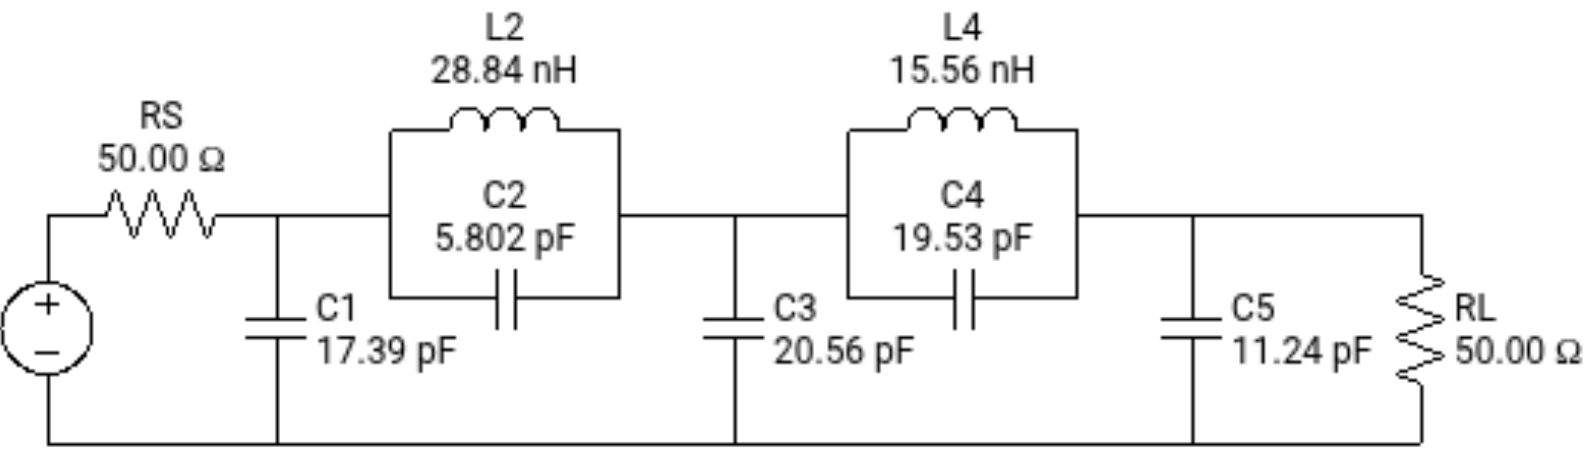
\includegraphics[width=0.8\linewidth]{images/passive_LC_Ladder_filter.png}
  \caption{Passive LC ladder impelementation (Large inductors)}
  \label{fig:passive_LC_Ladder_filter}
\end{figure}


\begin{figure}[htbp]
  \centering
  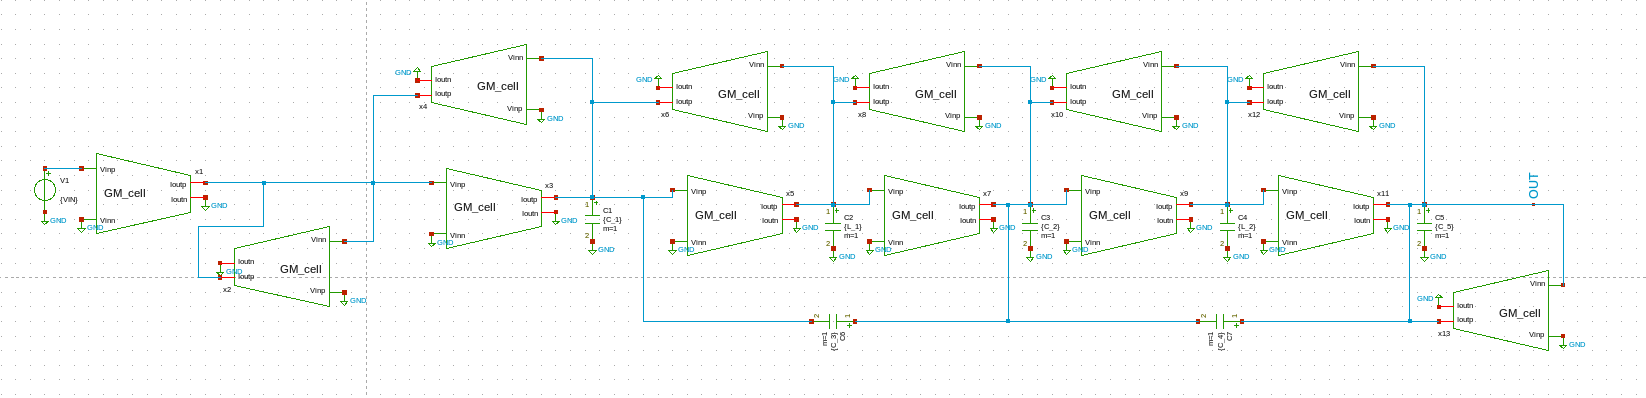
\includegraphics[width=1\linewidth]{images/GM_C_filter_simple_schem.png}
  \caption{Simplified schematic for GM-C filter}
  \label{fig:GM_C_filter_simple_schem}
\end{figure}

After choosing filter topology , required specifications for the 
GM-cell is specified using losses mapping technique discribed 
in \cite{Losses_mapping}, actually this technique benifit is 
very limited due to infinite quality factor of zeros, required
internisic gain of GM cell $\approx$ 200 , and integrated input-referred noise for the filter $\leq 99 \mu V$ RMS from 
equation~\ref{eq:noise_figure_input_noise}.

\subsection{GM-Cell Impelementation}%
\label{sub:GM-Cell Impelementation}
It's required to design a GM cell with low noise and high linearity
and AV $\approx$ 200 , because of high linearity , a large swing
output stage is required but non-dominant poles degrade quility
of the integrator
\subsubsection{Linearization technique}%
\label{ssub:Linearization technique}
First Linearization technique used is at filter level described
in \cite{linearization_techinque_filter} , the idea is described
be equation~\ref{eq:linearization_techinque} , this technique makes
differentail swing smaller for the input pairs which make third 
order non-linearity better at the cost of common-mode swing.
\begin{equation}
    GM(V_1^+ - V_1^-) - GM(V_3^+ - V_3^-)  = GM(V_1^+ - V_3^+) -
    GM(V_1^- - V_3^-)
    \label{eq:linearization_techinque}
\end{equation}

Second Linearization technique used is a simple resistive
degeneration  which degeades noise figure a little but improves 
linearity for input pairs descirbed by equation~\ref{eq:HD3_res_degen} \cite{resistive_degeneration} , where $N = gm\ RS$

\begin{equation}
    HD_3 = \frac{1}{32} \left[ \frac{v_{id}}{(1+N)(V_{dsat})} 
    \right]
    \label{eq:HD3_res_degen}
\end{equation}

\subsubsection{Proposed GM cell}%
Final GM-cell is shown in Figure~\ref{fig:GM_Cell}
\begin{figure}[htpb]
    \centering
    
\includegraphics[width=0.8\textwidth]{GM_cell.eps}
    \caption{Proposed GM cell architecture}
    \label{fig:GM_Cell}
\end{figure}

\clearpage
\section{Schematic Results}%

\subsection{GM cell Results}%
First simulation of GM-cell alone , paramters are shown in Table~\ref{tab:gm_cell_paramters}
\begin{table}[htpb]
    \centering
    \caption{GM cell Simulation results}
    \label{tab:gm_cell_paramters}

    \begin{tabular}{|c|c|}
        \hline
        Paramter &  Value \\ \hline
        DC gain (linear) & 170.5  \\ \hline
        Integrated input referred noise (up to 200MHz)
                         & 46.7 $\mu V$ \\ \hline
        GM & 25.86 mS \\ \hline
        Power Consumption & 21.11 mW \\ \hline
    \end{tabular}
\end{table}

\subsection{Filter AC results}%
Here are the AC and noise simulation results Figure~\ref{fig:FILTER-images-Filter_MAG_Response_OLD-pdf} and 
Figure~\ref{fig:group_delay}.
\begin{figure}[htpb]
    \centering
    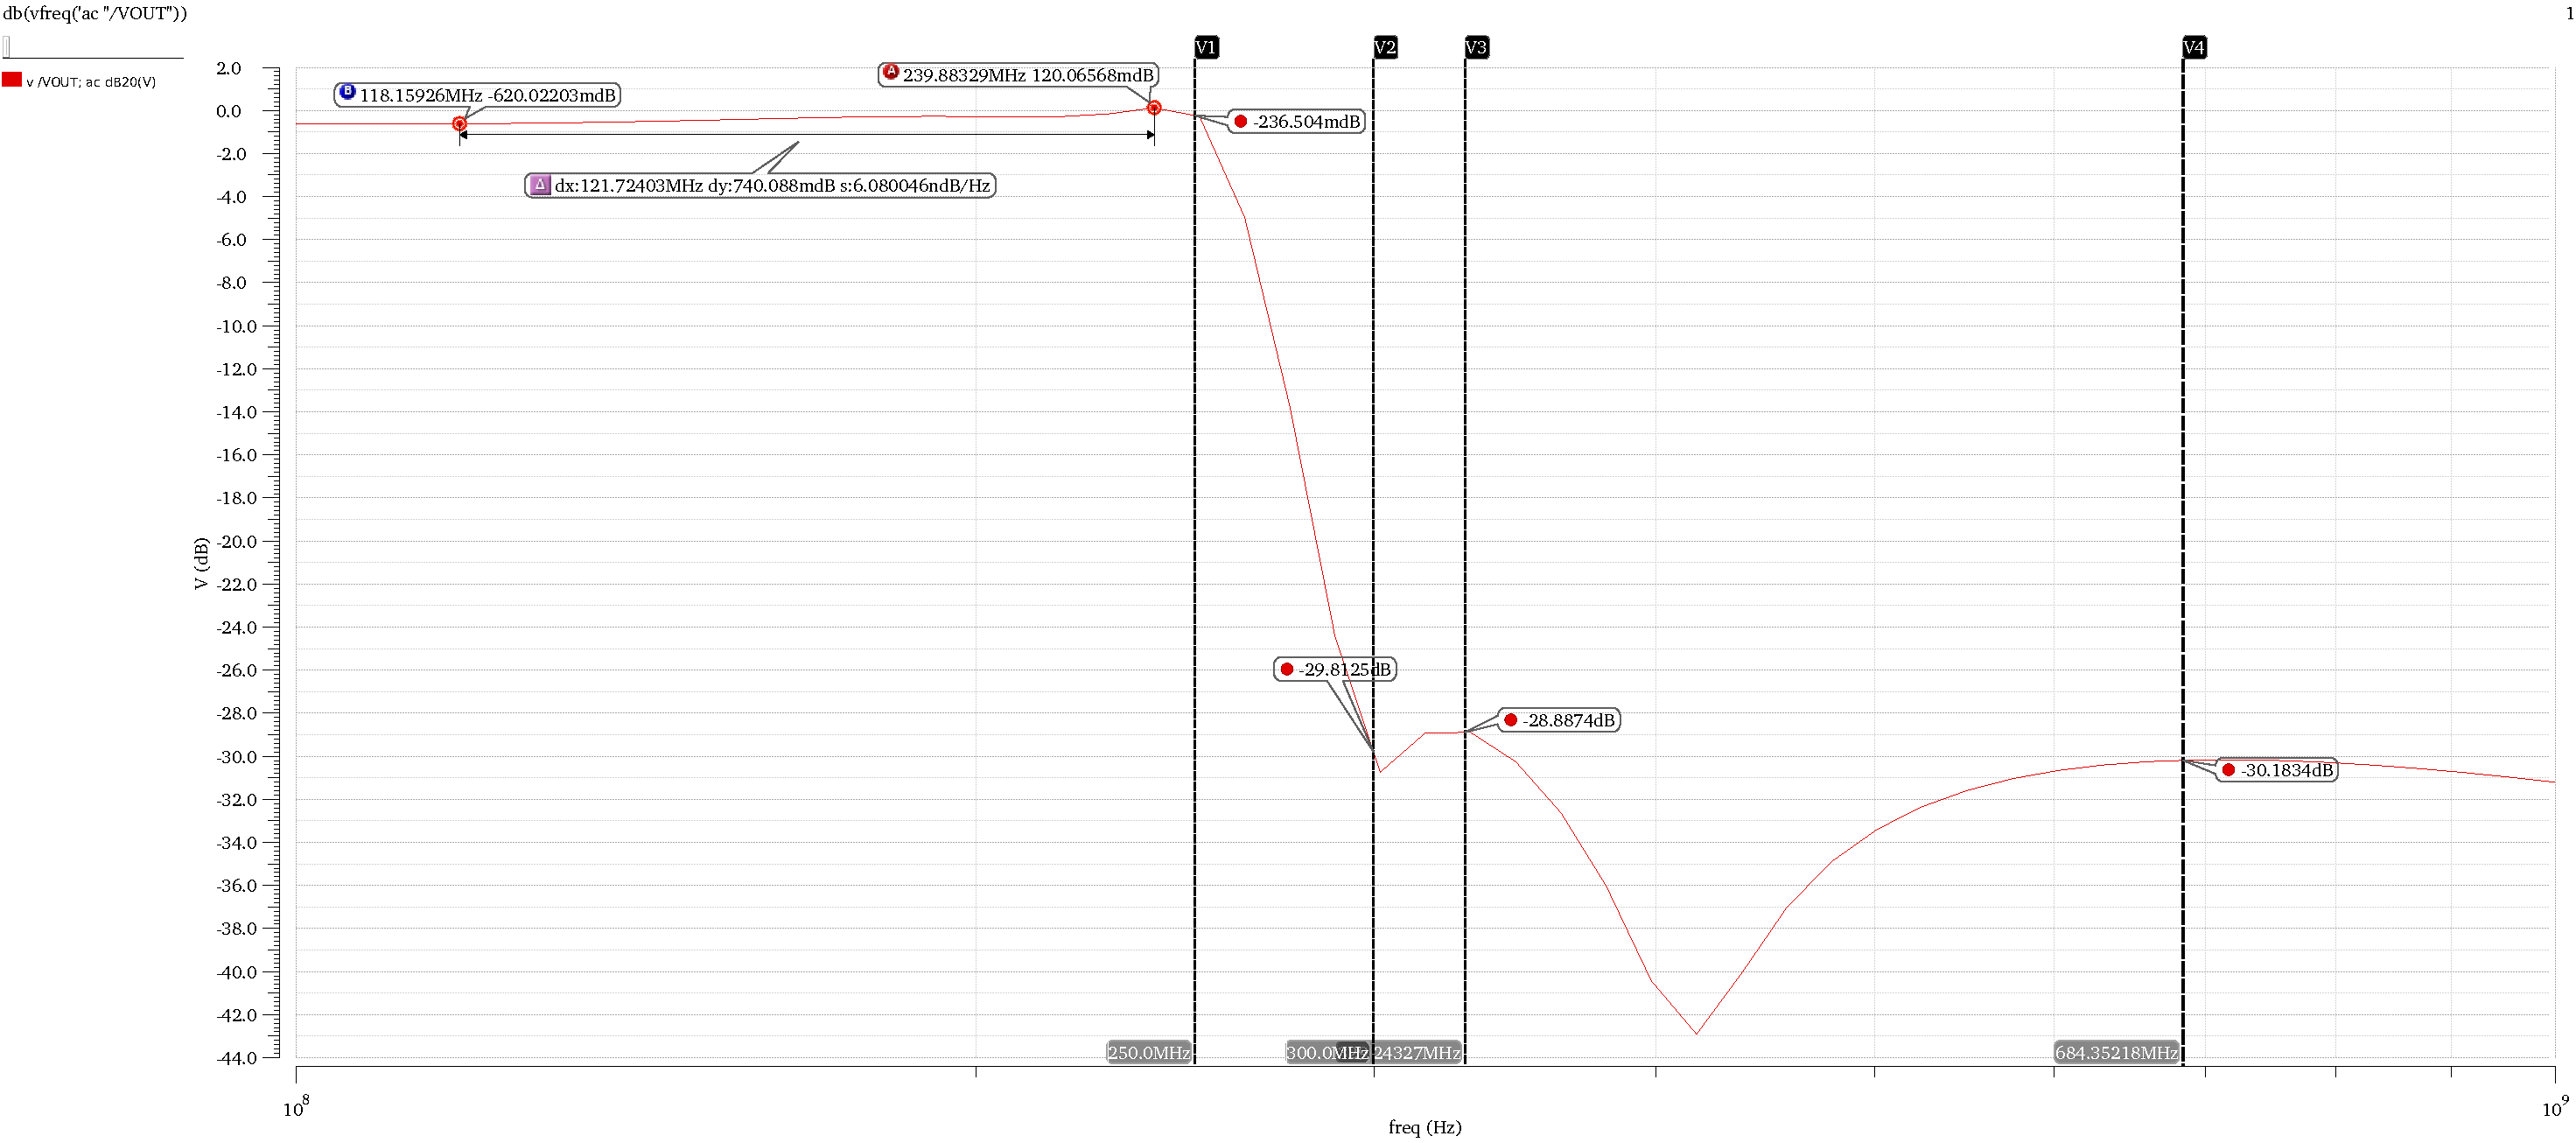
\includegraphics[width=1\textwidth]{FILTER/images/Filter_MAG_Response_OLD.pdf}
    \caption{Filter Magnitude response, 1dB-BW}
    \label{fig:FILTER-images-Filter_MAG_Response_OLD-pdf}
\end{figure}
\begin{figure}[htpb]
    \centering
    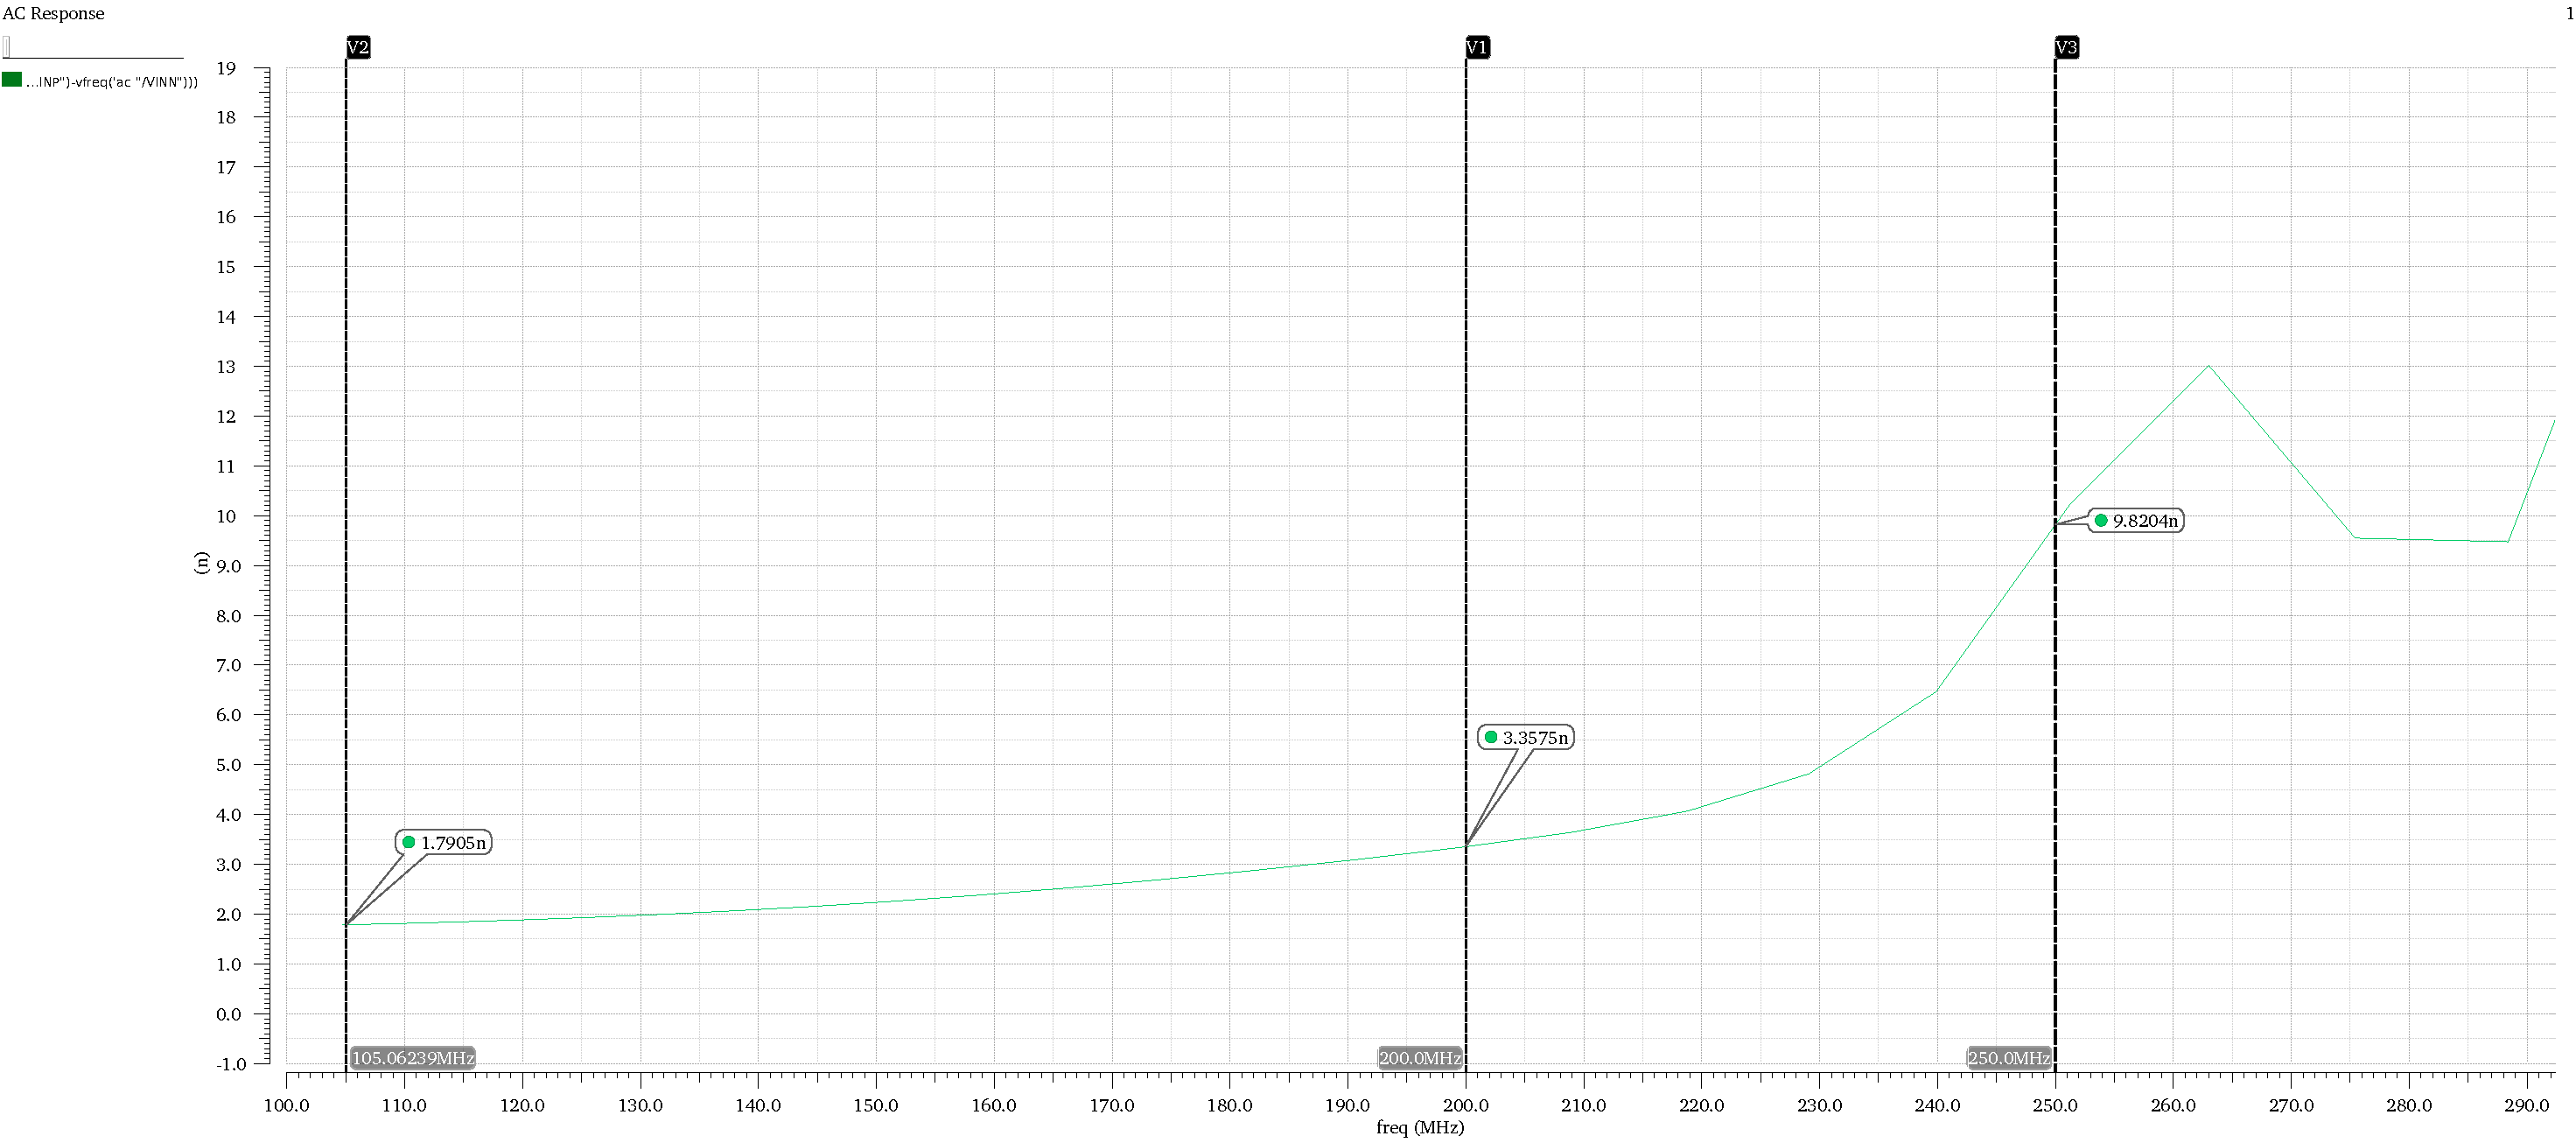
\includegraphics[width=1\textwidth]{FILTER/images/Filter_GD_ns_OLD.pdf}
    \caption{Group Delay: variation 1.56ns }
    \label{fig:group_delay}
\end{figure}

Integrated input referred noise up to 200MHz = 90.5$\mu V$ ,but 
full band 114.5$\mu V$ , suumary of AC results shown in 
Table~\ref{tab:filter_AC_summary}.
\begin{table}[htpb]
    \centering
    \caption{AC results summary}
    \label{tab:filter_AC_summary}

    \begin{tabular}{|c|c|}
        \hline
        Paramter& Value \\ \hline
        DC gain & -0.6 dB \\ \hline
        BW & 250 MHz  \\ \hline
        Rejection at 300MHz & -30 dB \\ \hline
        NF (up to 200MHz) & 11.25dB \\ \hline
        NF (total ) & 13.17dB \\ \hline
    \end{tabular}
\end{table}

\subsection{HB simulation}%
\label{sub:HB simulation}
For HB simulation two tones with 1mV peak amplitude is seperated by
10MHz are used.

As shown in Figure~\ref{fig:filter_oip3_vs_freq}, OIP3 varies very much with frequency , this is for two reasons ,
first is the filter response peaks with 
frequency ( High quality factor poles ) , second is the loop
gain for the GM cells degrades with frequency.
\begin{figure}[htpb]
    \centering
    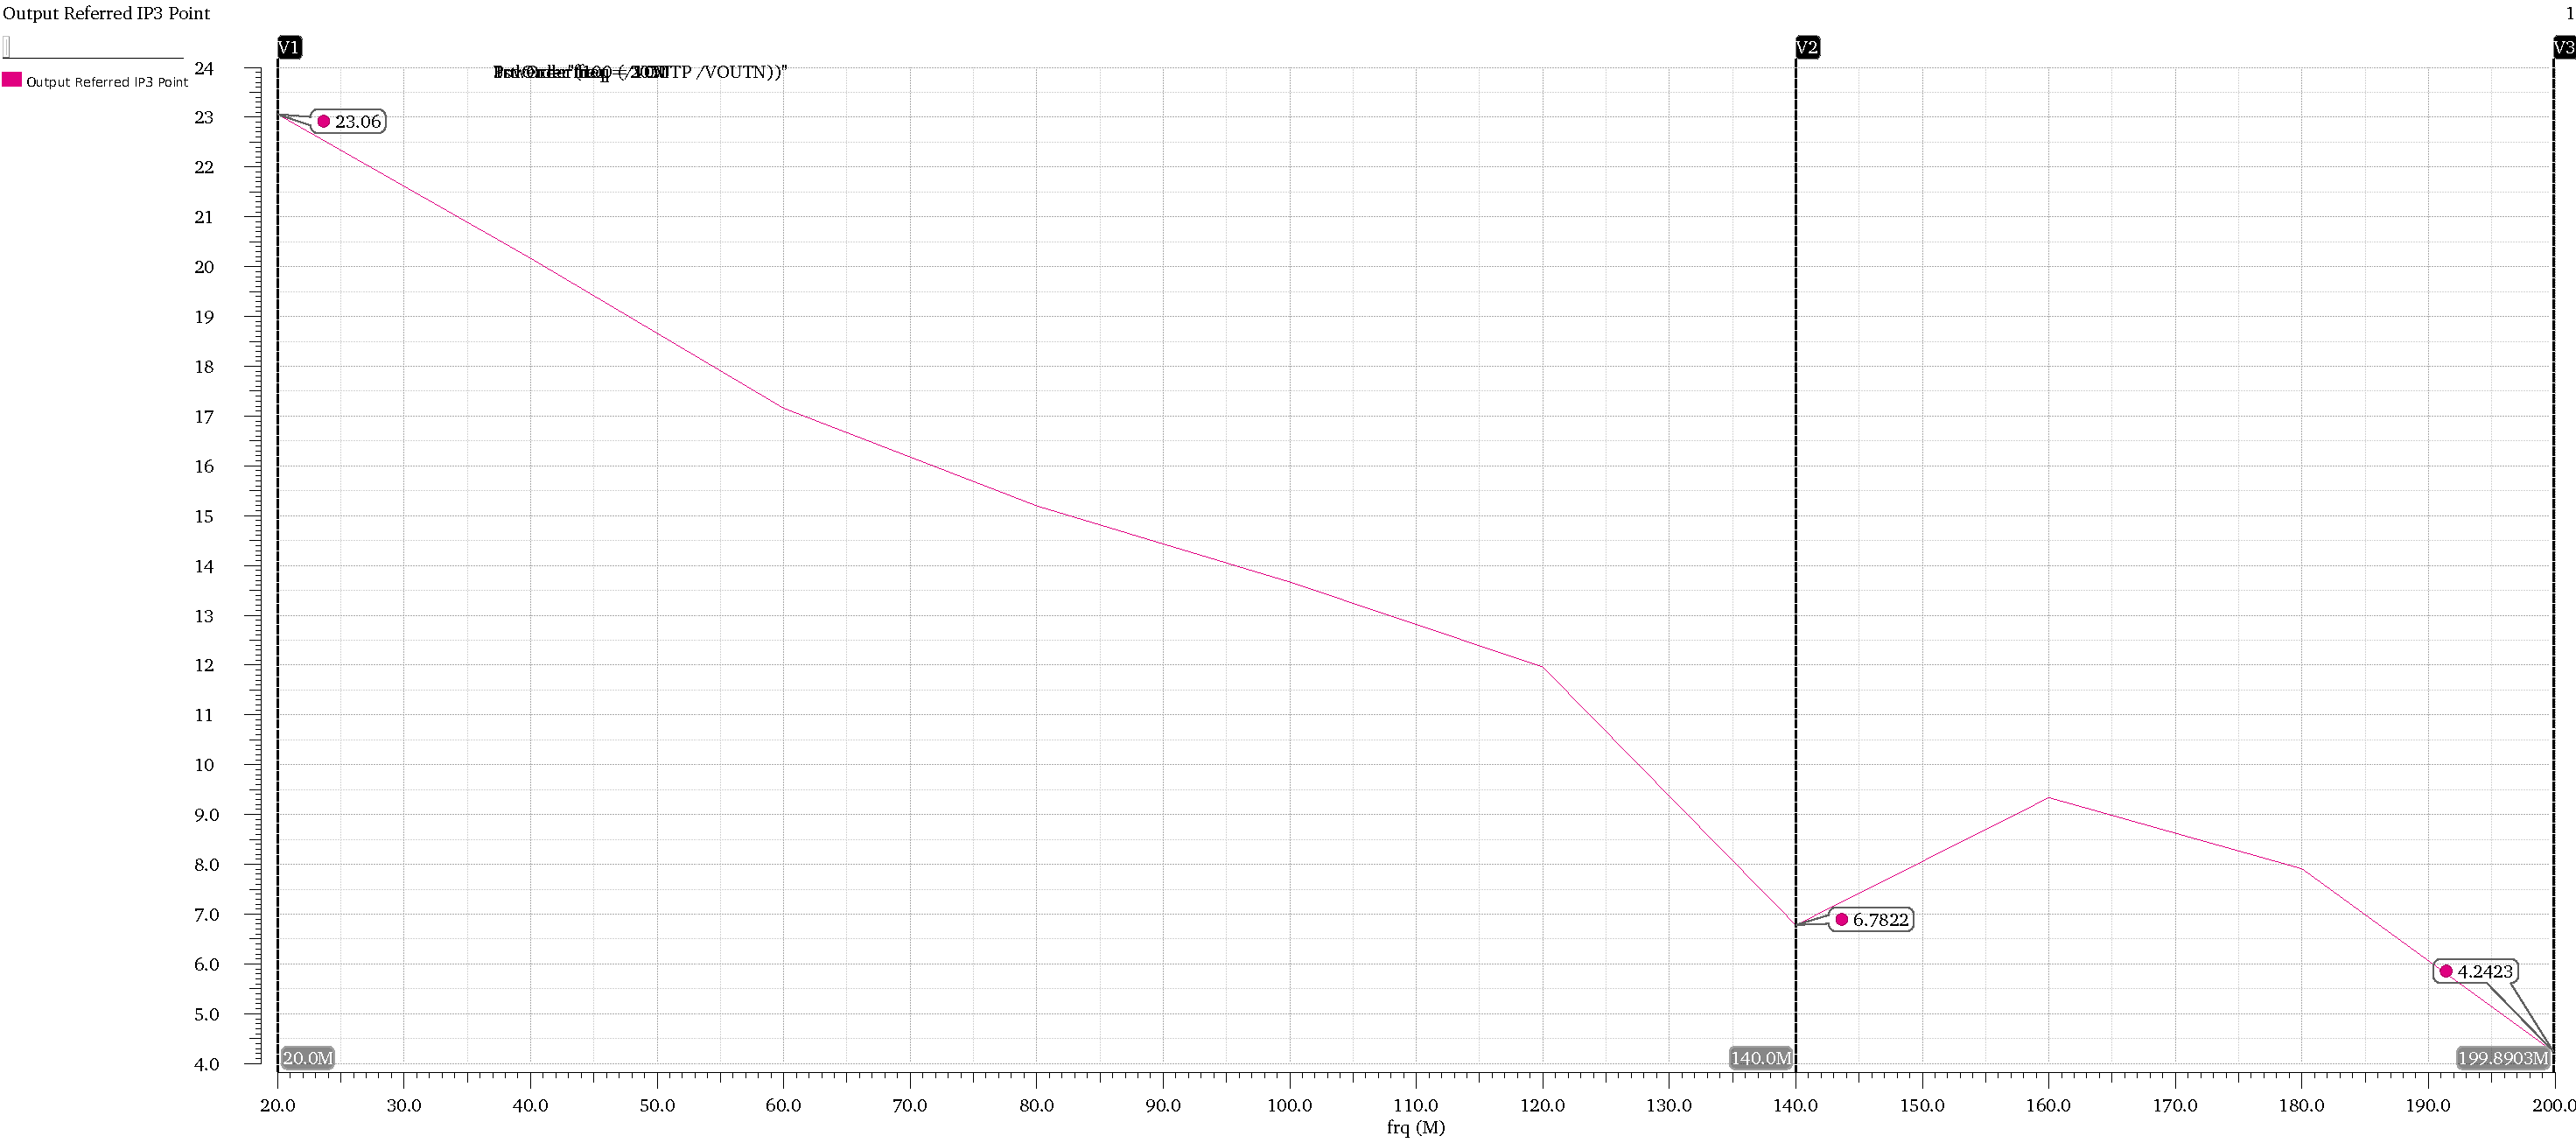
\includegraphics[width=1\textwidth]{FILTER/images/Filter_OIP3_Vs_freq_OLD.pdf}
    \caption{Filter OIP3 Vs frequency}
    \label{fig:filter_oip3_vs_freq}
\end{figure}
\begin{figure}[htpb]
    \centering
    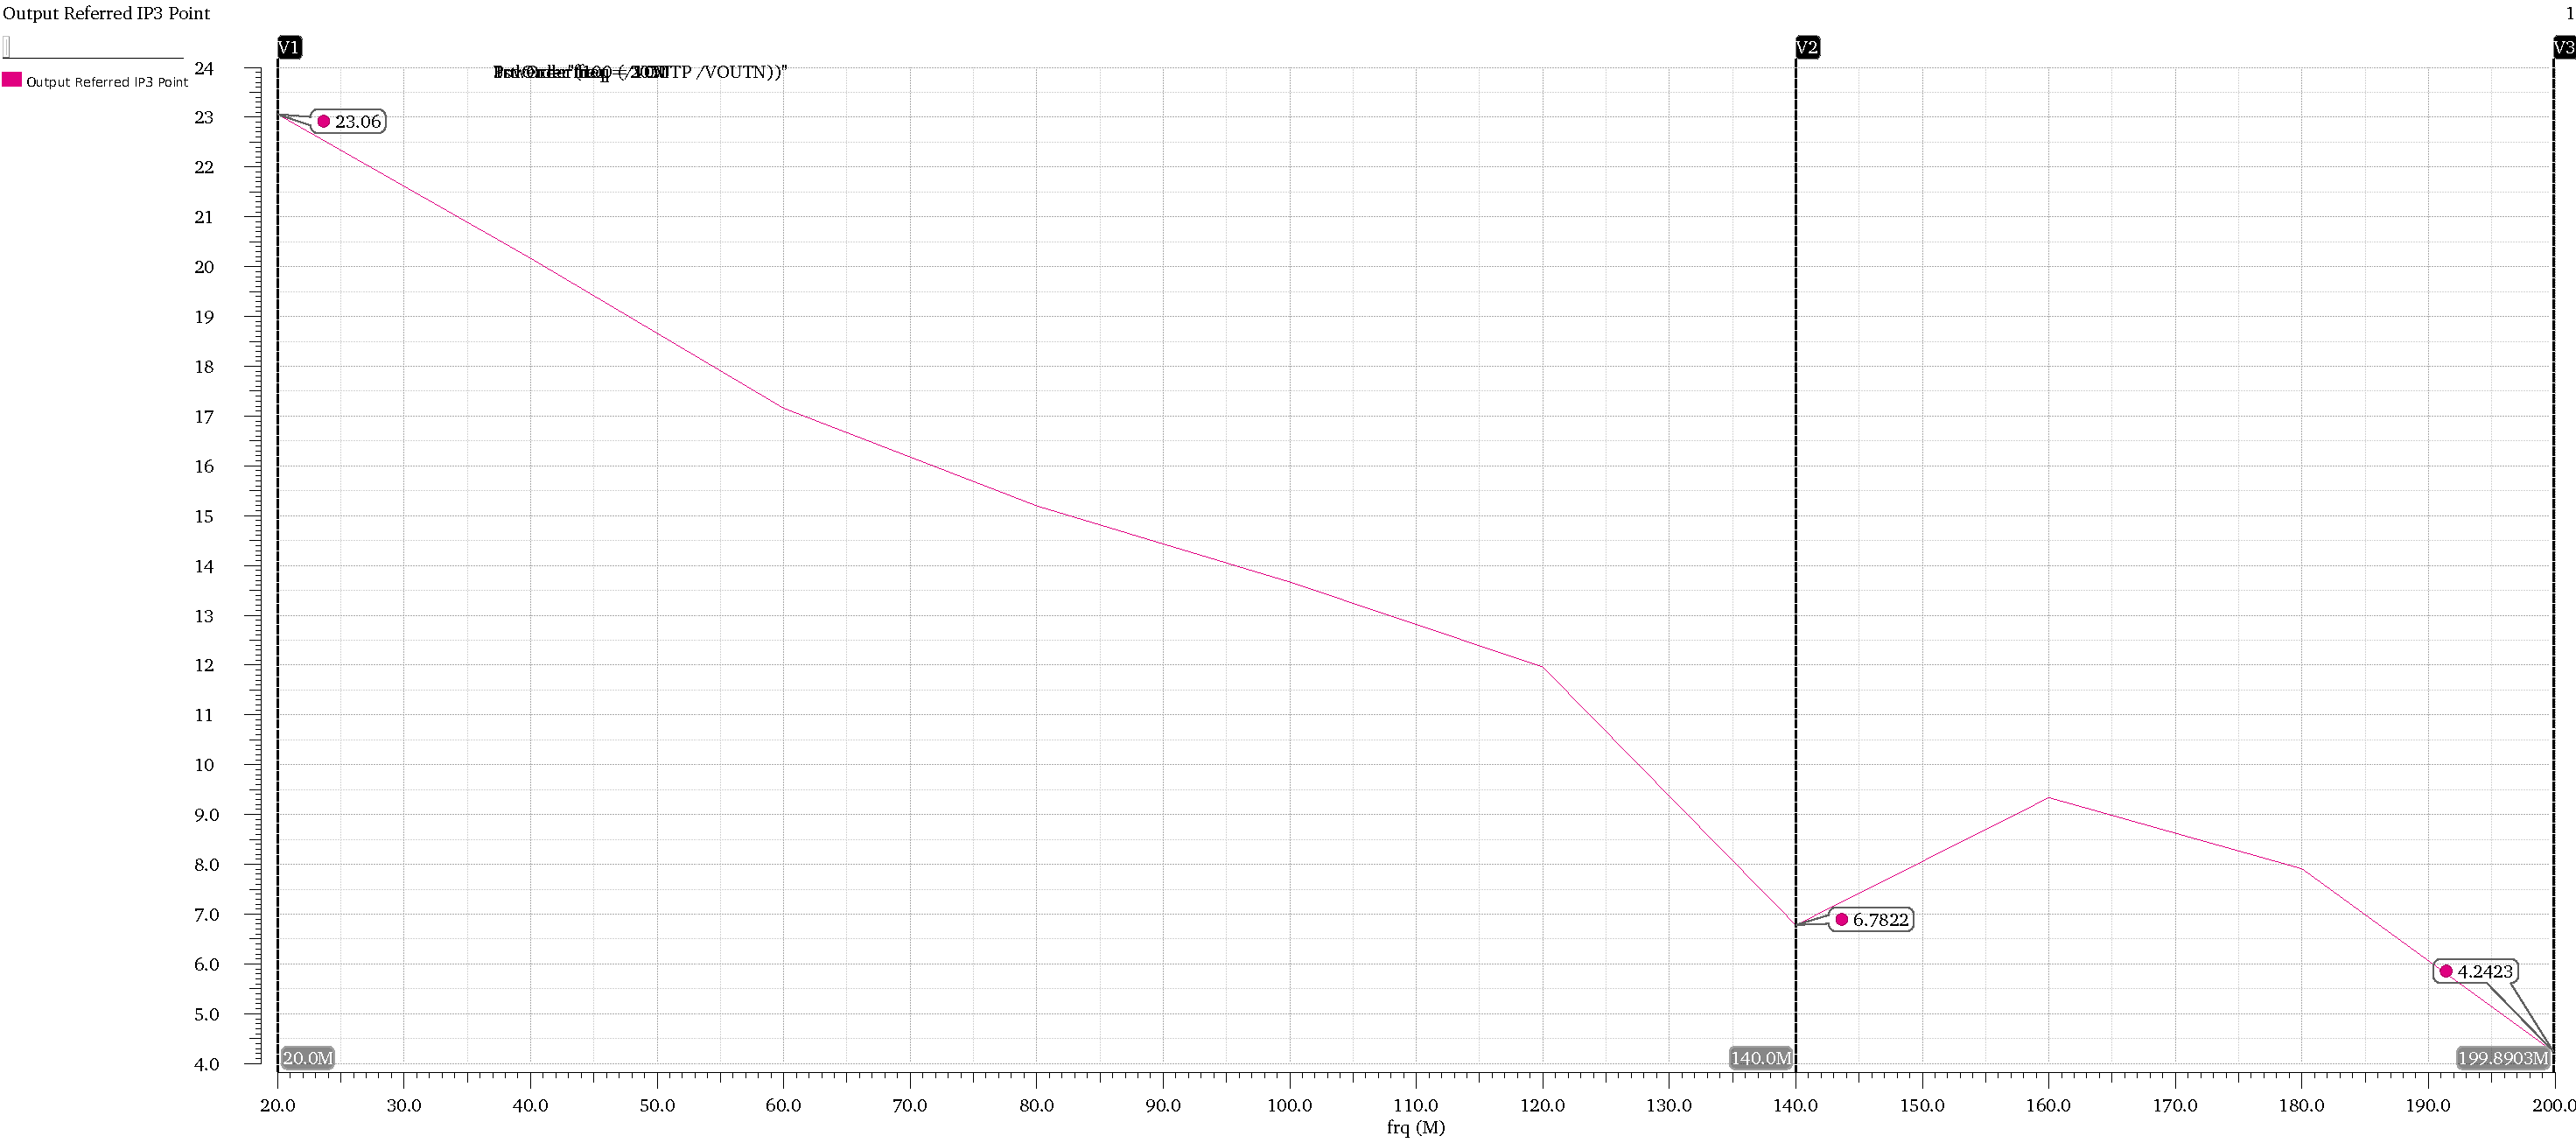
\includegraphics[width=1\textwidth]{FILTER/images/Filter_OIP3_Vs_freq_OLD.pdf}
    \caption{Filter OIP3 at 300MHz (blocker) and 200MHz (signal)}
    \label{fig:filter_oip3_blocker}
\end{figure}
\subsubsection{IP2 Results}%
\label{ssub:IP2 Results}
Monte carlo with mismatch is done to calculate OIP2 25 points only are used , small number of points are not very accurate 
\begin{figure}[htpb]
    \centering
    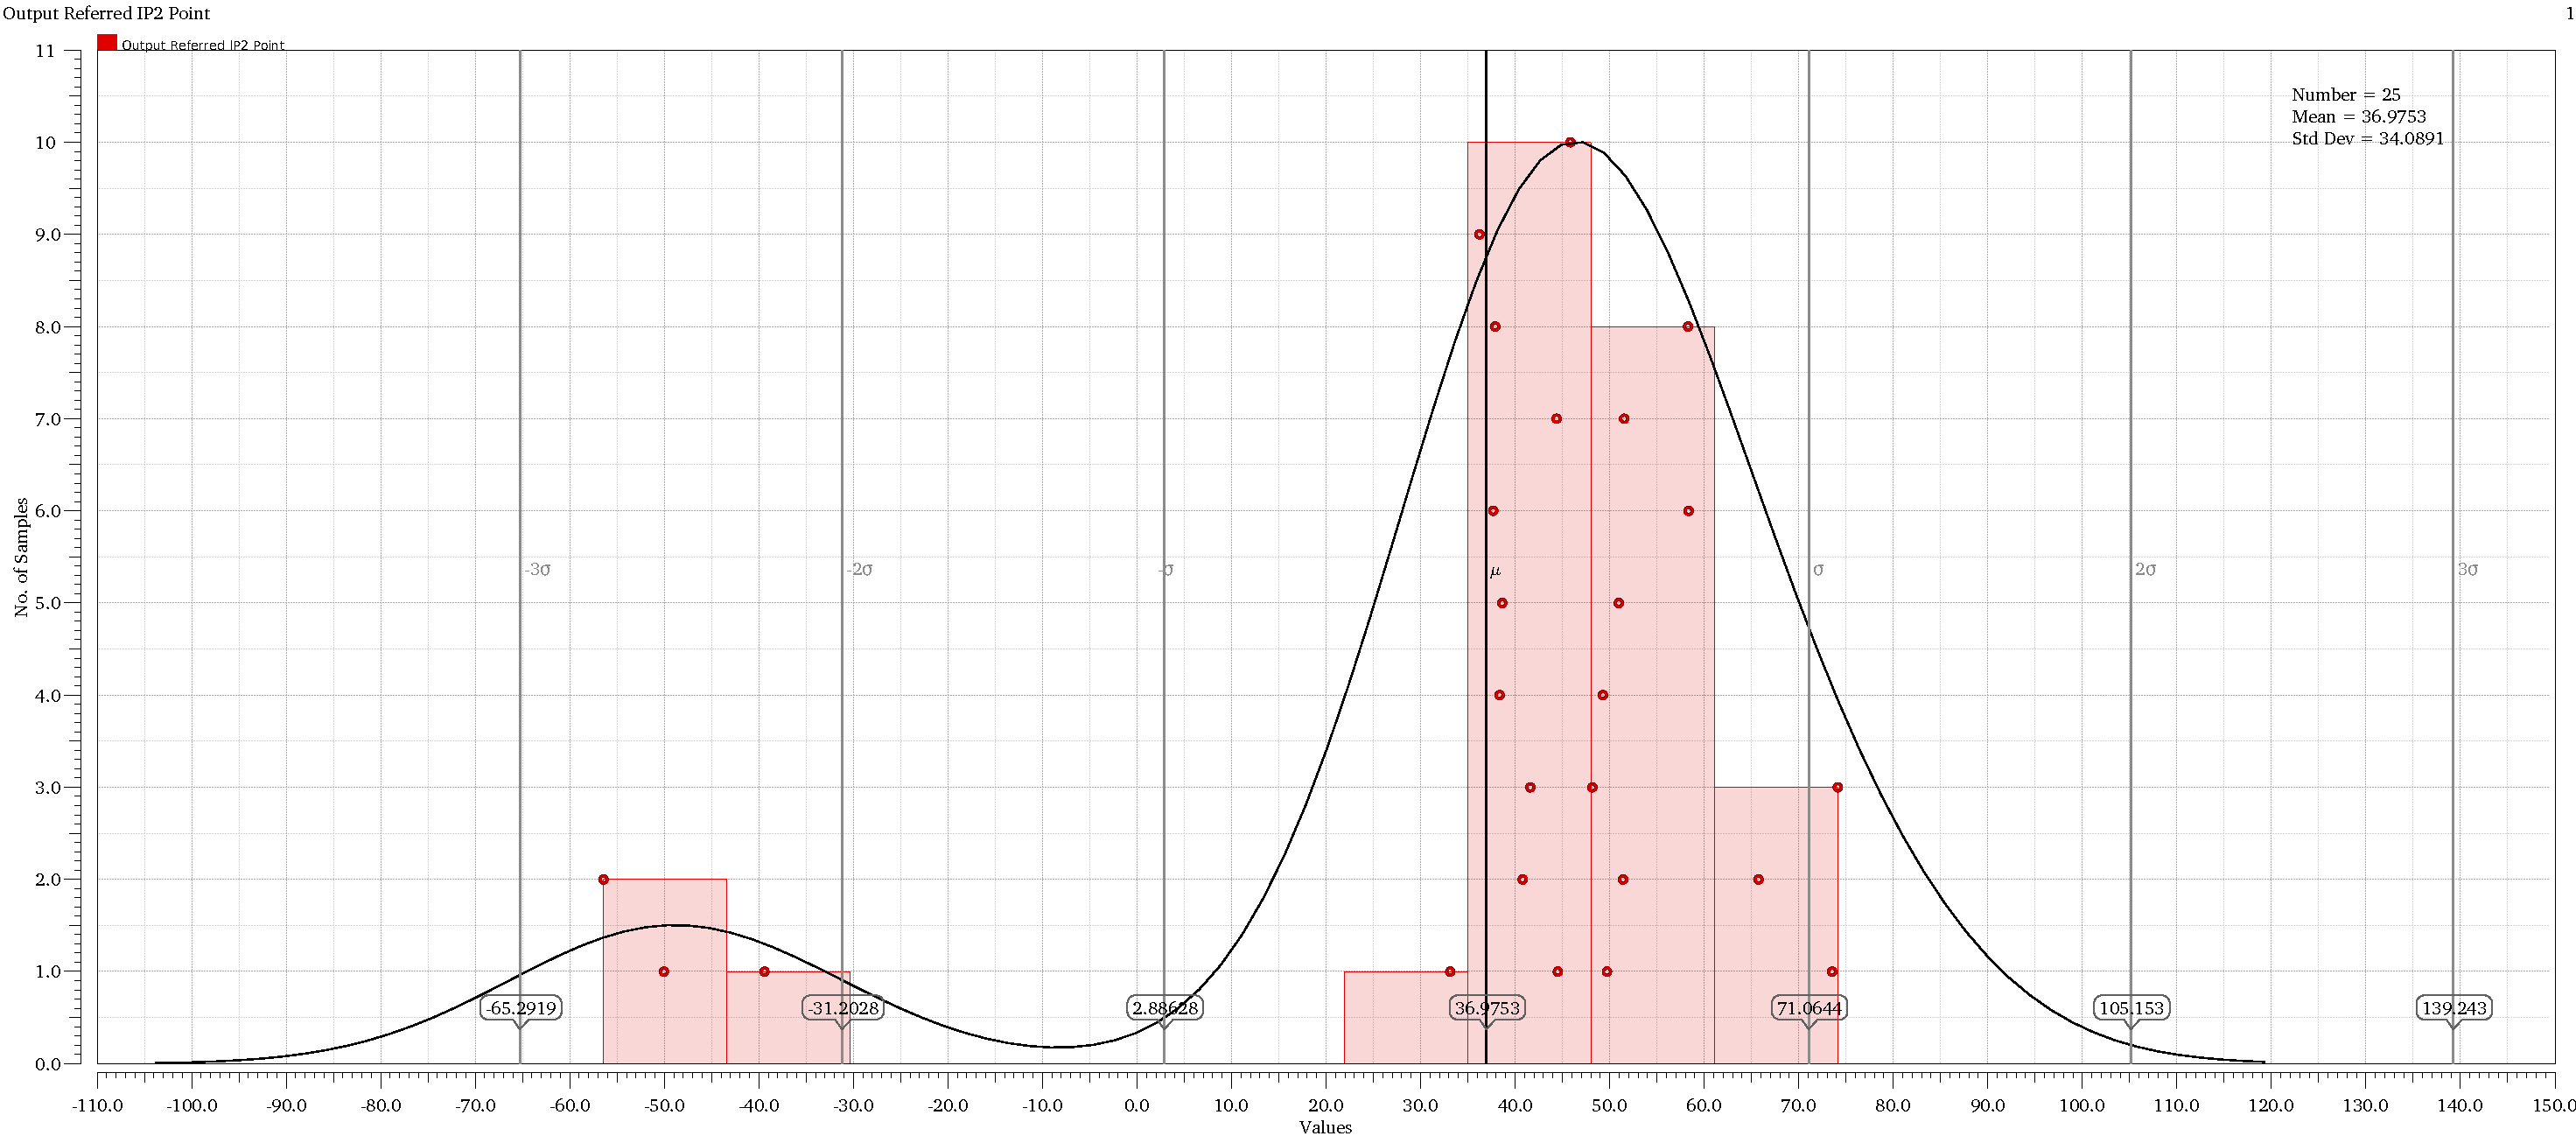
\includegraphics[width=1\textwidth]{FILTER/images/Filter_OIP2_200MHz_OLD.pdf}
    \caption{OIP2 monte carlo (25 point), mean = 37dBm}
    \label{fig:oip2_monte_carlo}
\end{figure}


\subsection{Corners}%
\label{sub:Corners}
It's clear from Figure~\ref{fig:filter_corners} that GM-C filter
Bandwidth depends on GM itself which changes with corners ,
trimming with degeneration resistance is required to maintain
constant GM across corners , so it's useless to proceed with 
corners simulations now
\begin{figure}[htpb]
    \centering
    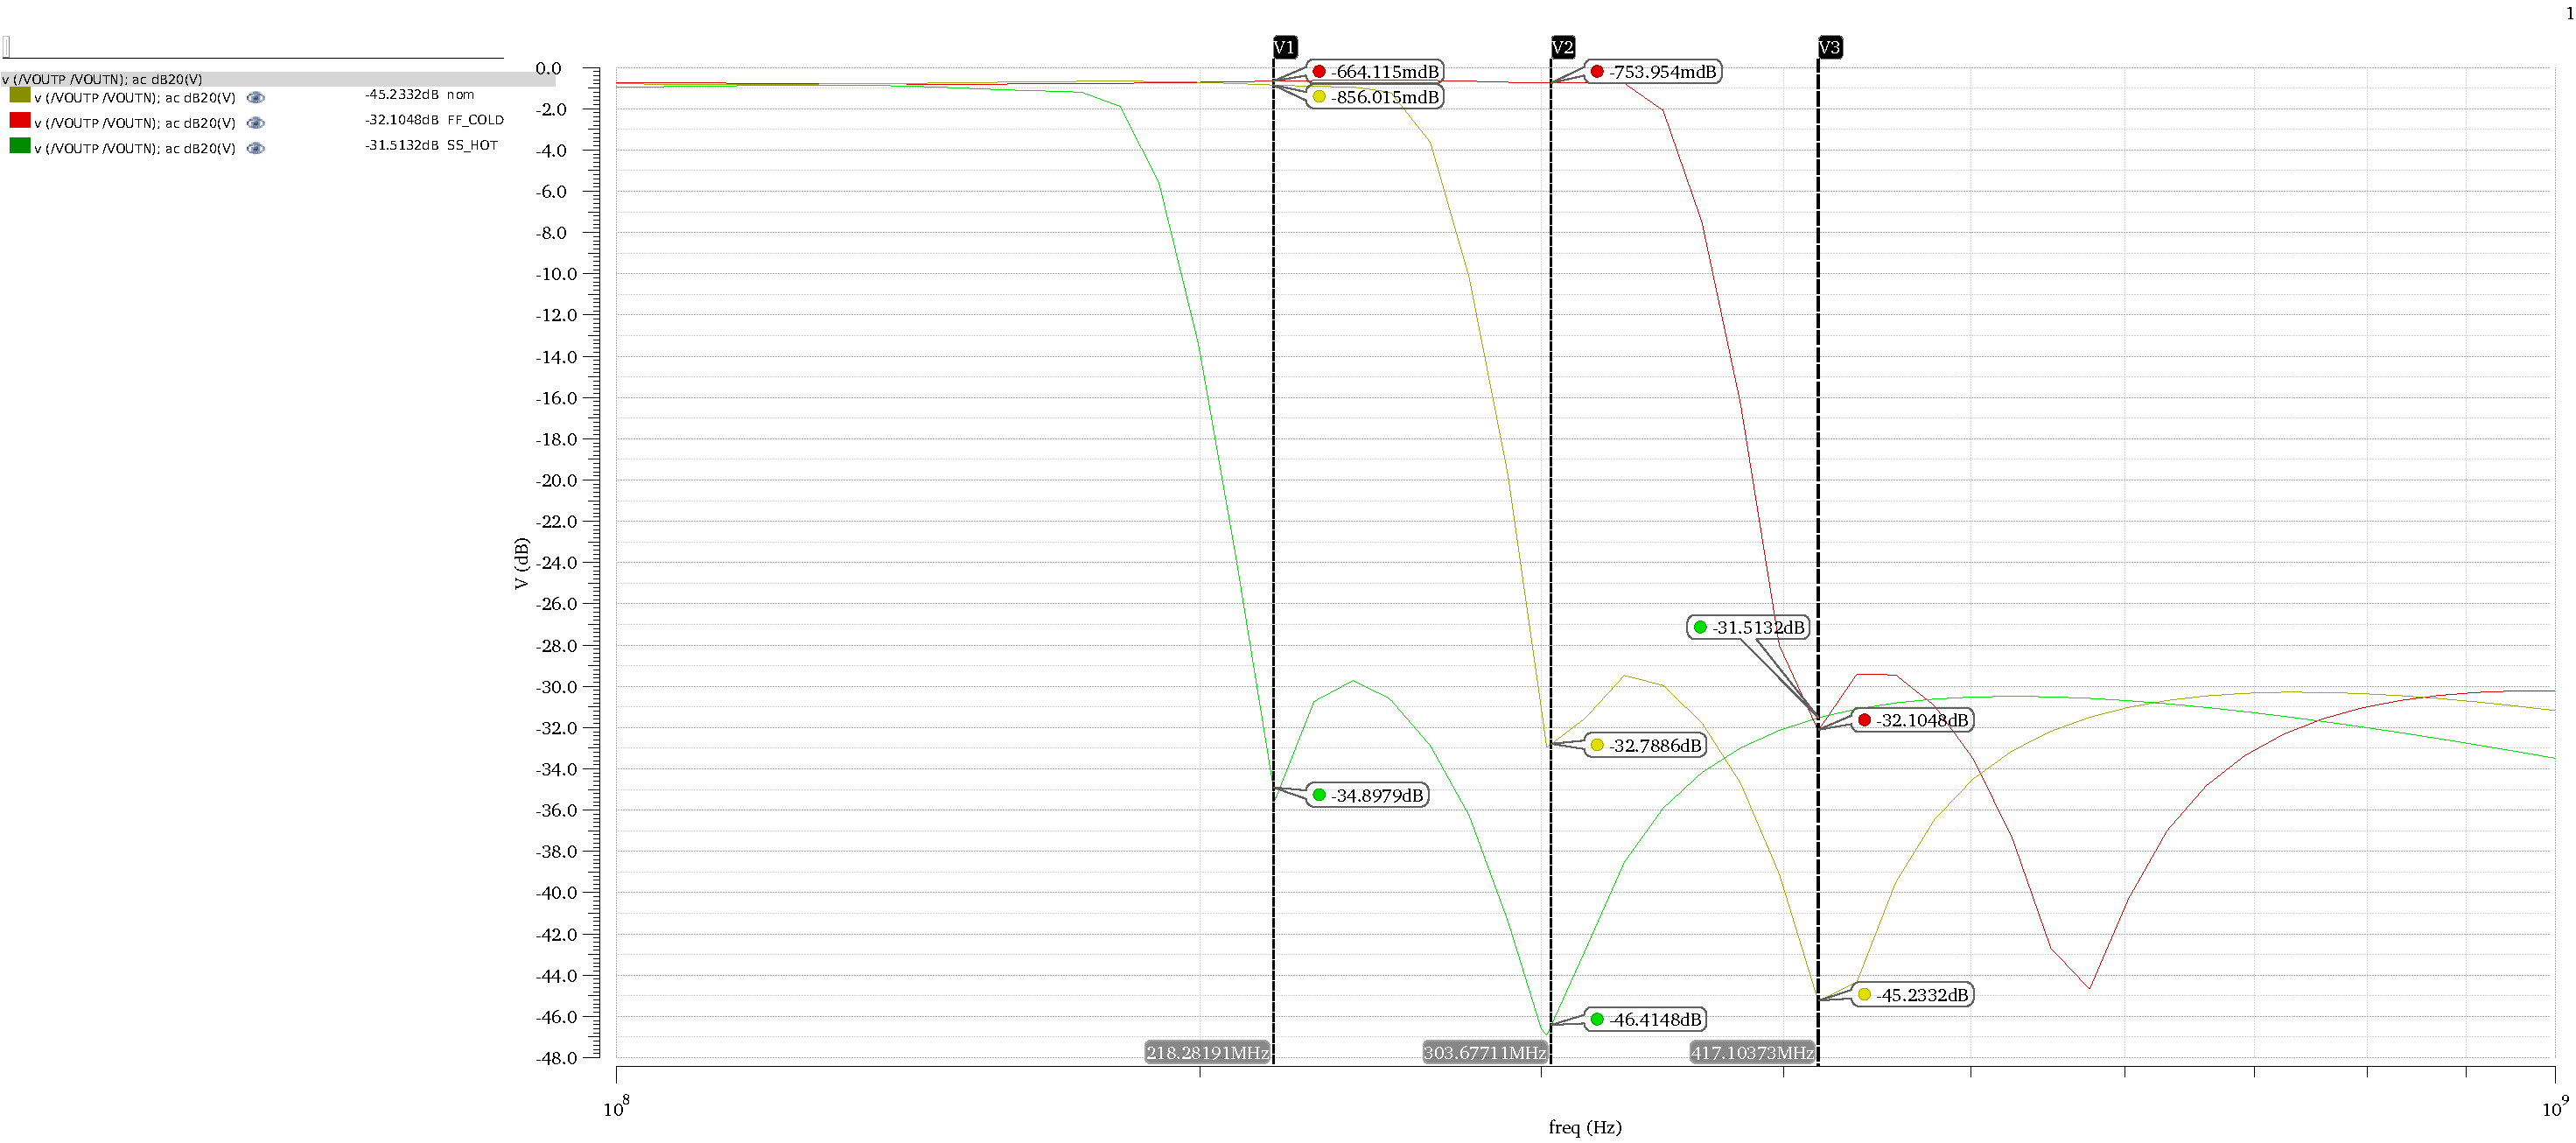
\includegraphics[width=1\textwidth]{FILTER/images/Filter_MAG_Response_corners.pdf}
    \caption{Filter Magnitude response Vs corners}
    \label{fig:filter_corners}
\end{figure}
\subsection{Summary}%
The filter shows a serious problem with linearity variation with
frequency, layout of the filter is missing.
\begin{table}[htpb]
    \centering
    \caption{Achieved Specifications}
    \label{tab:filter_specs_achieved}
    \begin{tabular}{l c c}
        \toprule
    \textbf{Paramter} & \textbf{Specifications} & 
    \textbf{Achieved} \\ \hline
    Gain & 0 dB & -0.6 dB \\ \hline
    BW & 250 MHz &  250 MHz \\ \hline
    NF & 12 dB & 11.25 dB (13.17 dB) \\ \hline
    IIP3 & 16 dBm & 4.24 dBm \\ \hline
    Power Consumption & & 295mW \\ \hline
    Supply & & 1.6V \\ \bottomrule
    \end{tabular}
\end{table}
%\begin{table}[htbp]
%    \centering
%    \label{tab:original_specs}
%    \caption{Receiver Chain Block Specifications}
%    % \textwidth forces the table to fit your exact page margins
%    \begin{tabularx}{\textwidth}{l c c c X} 
%        \toprule
%        \textbf{Block} & \textbf{Gain} & \textbf{Noise Figure} & \textbf{OIP3} & \textbf{Other Specs} \\ 
%        \midrule
%        First LNA (External)  & 20 dB & 2 dB & 35 dBm & \\ 
%        Second LNA (Internal) & 14 dB & 3 dB & 33 dBm & \\ 
%        DSA                   & -3 dB & 3 dB & 33 dBm & Control range = 15 dB \\ 
%        Mixer                 & -7 dB & 7 dB & 15 dBm & \\ 
%        LPF                   & -2 dB & 2 dB & 34 dBm & 0.5\,dB-BW = 250\,MHz, \newline 3\,dB-BW = 600\,MHz \\ 
%        \bottomrule
%    \end{tabularx}
%\end{table}
%
%
















